\subsection{EPC Page Eviction}
\label{sec:sgx_epc_eviction}

Modern OS kernels take advantage of address translation~(\S~\ref{sec:paging})
to implement page swapping, also referred to as paging~(\S~\ref{sec:paging}).
In a nutshell, paging allows the OS kernel to over-commit the computer's DRAM
by evicting rarely used memory pages to a slower storage medium that is
referred to as the disk.

Paging is a key contributor to utilizing a computer's resources effectively.
For example, a desktop system whose user runs multiple programs concurrently
can evict memory pages allocated to inactive applications without a significant
degradation in user experience.

Unfortunately, the OS cannot be allowed to evict an enclave's EPC pages via the
same methods that are used to implement page swapping for DRAM memory outside
the PRM range. In the SGX threat model, enclaves do not trust the system
software, so the SGX design offers an EPC page eviction method that can defend
against a malicious OS that attempts any of the active address translation
attacks described in \S~\ref{sec:address_translation_attacks}.

The price of the security afforded by SGX is that an OS kernel that supports
evicting EPC pages must use a modified page swapping implementation that
interacts with the SGX mechanisms. Enclave authors can mostly ignore EPC
evictions, similarly to how today's application developers can ignore the OS
kernel's paging implementation.

As illustrated in Figure~\ref{fig:sgx_page_eviction}, SGX supports evicting
EPC pages to DRAM pages outside the PRM range. The system software is expected
to use its existing page swapping implementation to evict the contents of these
pages out of DRAM and onto a disk.

\begin{figure}[hbt]
  \centering
  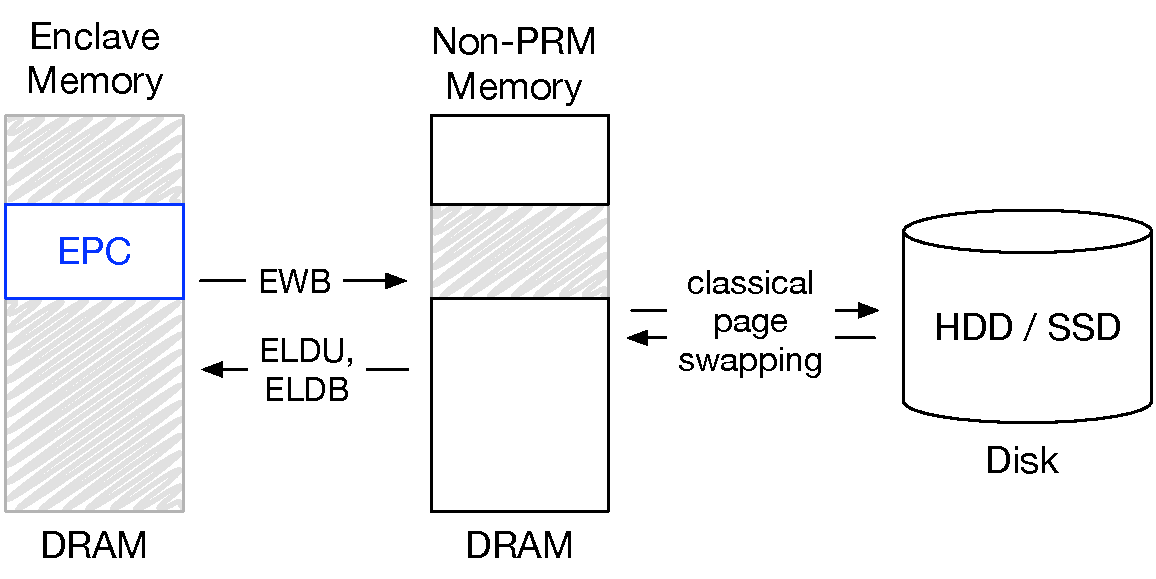
\includegraphics[width=85mm]{figures/sgx_page_eviction.pdf}
  \caption{
    SGX offers a method for the OS to evict EPC pages into non-PRM DRAM. The
    OS can then use its standard paging feature to evict the pages out of DRAM.
  }
  \label{fig:sgx_page_eviction}
\end{figure}

SGX's eviction feature revolves around the \texttt{EWB} instruction, described
in detail in \S~\ref{sec:sgx_ewb}. Essentially, \texttt{EWB} evicts an EPC page
into a DRAM page outside the EPC and marks the EPC page as available, by
zeroing the VALID field in the page's EPCM entry.

The SGX design relies on symmetric key cryptograpy~\ref{sec:crypto_keys} to
guarantee the privacy and integrity of the evicted EPC pages, and on
nonces~(\S~\ref{sec:freshness_crypto}) to guarantee the freshness of the pages
brought back into the EPC. These nonces are stored in Version Arrays~(VAs),
covered in \S~\ref{sec:sgx_va}, which are EPC pages dedicated to nonce storage.

Before an EPC page is evicted and freed up for use by other enclaves, the SGX
implementation must ensure that no TLB has address translations associated with
the evicted page, in order to avoid the TLB-based address translation attack
described in \S~\ref{sec:tlb_mapping_attacks}.

As explained in \S~\ref{sec:sgx_epc}, SGX leaves the system software in charge
of managing the EPC. It naturally follows that the SGX instructions described
in this section, which are used to implement EPC paging, are only available to
system software, which runs at ring 0~\S~\ref{sec:rings}.

In today's software stacks~(\S~\ref{sec:rings}), only the OS kernel implements
page swapping in order to support the over-committing of DRAM. The hypervisor
is only used to partition the computer's physical resources between operating
systems. Therefore, this section is written with the expectation that the OS
kernel will also take on the responsibility of EPC page swapping. For
simplicity, we often use the term ``OS kernel'' instead of ``system software''.
The reader should be aware that the SGX design does not preclude a system where
the hypervisor implements its own EPC page swapping. Therefore, ``OS kernel''
should really be read as ``the system software that performs EPC paging''.


\subsubsection{Page Eviction and the TLBs}
\label{sec:sgx_eblock}

One of the least promoted accomplishments of SGX is that it does not add any
security checks to the memory execution units~(\S~\ref{sec:cpu_core},
\S~\ref{sec:out_of_order}). Instead, SGX's access control checks occur after an
address translation~(\S~\ref{sec:paging}) is performed, right before the
translation result is written into the TLBs~(\S~\ref{sec:tlbs}). This aspect
is generally downplayed throughout the SDM, but it becomes visible when
explaining SGX's EPC page eviction mechanism.

A full discussion of SGX's access control checks merits its own section, and is
defered to \S~\ref{sec:xxx}. The EPC page eviction mechanisms can be explained
using only two requirements from SGX's security model. First, when a logical
processor exits an enclave, either via
\texttt{EEXIT}~(\S~\ref{sec:sgx_eexit}) or via an AEX~(\S~\ref{sec:sgx_aex}),
its TLBs are flushed. Second, when an EPC page is deallocated from an enclave,
all logical processors executing that enclave's code must be directed to exit
the enclave. This is sufficient to guarantee the removal of any TLB entry
targeting the deallocated EPC.

System software can cause a logical processor to exit an enclave by sending it
an Inter-Processor Interrupt (IPI,~\S~\ref{sec:interrupts}), which will trigger
an AEX when received. Essentially, this is a very coarse-grained TLB shootdown.

SGX does not trust system software. Therefore, before marking an EPC page's
EPCM entry as free, the SGX implementation must ensure that the OS kernel has
flushed all the TLBs that might contain translations for the page. Furthermore,
performing IPIs and TLB flushes for each page eviction would add a significant
overhead to a paging implementation, so the SGX design allows a batch of pages
to be evicted using a single IPI / TLB flush sequence.

% Enclave Page Cache Map (EPCM): SDM S 38.19

The TLB flush verification logic relies on a 1-bit EPCM entry field called
BLOCKED. As shown in Figure~\ref{fig:sgx_page_states}, the VALID and BLOCKED
fields yield three possible EPC page states. A page is \textit{free} when both
bits are zero, \textit{in use} when VALID is zero and BLOCKED is one, and
\textit{blocked} when both bits are one.

\begin{figure}[hbt]
  \centering
  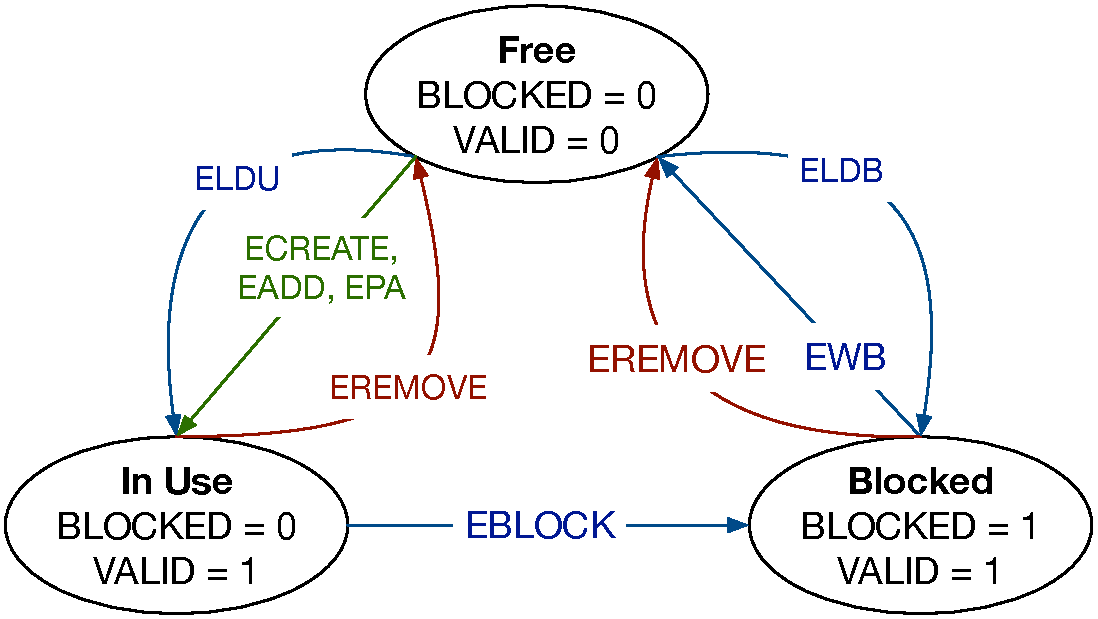
\includegraphics[width=80mm]{figures/sgx_page_states.pdf}
  \caption{
    The VALID and BLOCKED bits in an EPC page's EPCM entry can be in one of
    three states. \texttt{EADD} and its siblings allocate new EPC pages.
    \texttt{EREMOVE} permanently deallocates an EPC page. \texttt{EBLOCK}
    blocks an EPC page so it can be evicted using \texttt{EWB}.\texttt{ELDB}
    and \texttt{ELDU} load an evicted page back into the EPC.
  }
  \label{fig:sgx_page_states}
\end{figure}

Blocked pages are not considered accessible to enclaves. If an address
translation results in a blocked EPC page, the SGX implementation causes the
translation to result in a Page Fault~(\#PF,~\S~\ref{sec:faults}). This
guarantees that once a page is blocked, the CPU will not create any new TLB
entries pointing to it.

Furthermore, every SGX instruction makes sure that the EPC pages that it
operates on are not blocked. For example, \texttt{EENTER} ensures that the TCS
it is given is not blocked, that its enclave's SECS is not blocked, and that
every page in the current SSA is not blocked.

% Eviction of Enclave Pages: SDM S 39.5.3

In order to evict a batch of EPC pages, the OS kernel must first issue
\texttt{EBLOCK} instructions targeting them. The OS is also expected to remove
the EPC page's mapping from page tables, but is not trusted to do so.

After all the desired pages have been blocked, the OS kernel must execute an
\texttt{ETRACK} instruction, which directs the SGX implementation to keep track
of which logical processors have had their TLBs flushed. \texttt{ETRACK}
requires the virtual address of an enclave's SECS~(\S~\ref{sec:sgx_secs}). If
the OS wishes to evict a batch of EPC pages belonging to multiple enclaves, it
must issue an \texttt{ETRACK} for each enclave.

Following the \texttt{ETRACK} instructions, the OS kernel must induce enclave
exits on all the logical processors that are executing code inside the enclaves
that have been \texttt{ETRACK}ed. The SGX design expects that the OS will use
IPIs to cause AEXes in the logical processors whose TLBs must be flushed.

The EPC page eviction process is completed when the OS executes an \texttt{EWB}
instruction for each EPC page to be evicted. This instruction, which will be
fully described in \S~\ref{sec:sgx_ewb}, writes an encrypted version of the EPC
page to be evicted into DRAM, and then frees the page by clearing the VALID and
BLOCKED bits in its EPCM entry. Before carrying out its tasks, \texttt{EWB}
ensures that the EPC page that it targets has been blocked, and checks the
state set up by \texttt{ETRACK} to make sure that all the relevant TLBs have
been flushed.

An evicted page can be loaded back into the EPC via the \texttt{ELDU} and
\texttt{ELDB} instructions. Both instructions start up with a free EPC page and
a DRAM page that has the evicted contents of an EPC page, decrypt the DRAM
page's contents into the EPC page, and restore the corresponding EPCM entry.
The only difference between \texttt{ELDU} and \texttt{ELDB} is that the latter
sets the BLOCKED bit in the page's EPCM entry, whereas the former leaves it
cleared.

\texttt{ELDU} and \texttt{ELDB} resemble \texttt{ECREATE} and \texttt{EADD},
in the sense that they populate a free EPC page. Since the page that they
operate on was free, the SGX security model predicates that no TLB entries can
possibly target it. Therefore, these instructions do not require a mechanism
similar to \texttt{EBLOCK} or \texttt{ETRACK}.


\subsubsection{The Version Array (VA)}
\label{sec:sgx_va}
\label{sec:sgx_epa}

% Version Array (VA): SDM S 38.18
% EPC and Management of EPC Pages: SDM S 39.5, 39.5.{2,3,4,5,6}

When \texttt{EWB} evicts the contents of an EPC, it creates an 8-byte
nonce~(\S~\ref{sec:freshness_crypto}) that Intel's documentation calls a
\textit{page version}. SGX's freshness guarantees are built on the assumption
that nonces are stored securely, so \texttt{EWB} stores the nonce that it
creates inside a \textit{Version Array}~(VA).

Version Arrays are EPC pages that are dedicated to storing nonces generated by
EWB. Each VA is divided into slots, and each slot is exactly large enough to
store one nonce. Given that the size of an EPC page is 4KB, and each nonce
occupies 8 bytes, it follows that each VA has 512 slots.

% EPA: SDM S 41.3

VA pages are allocated using the \texttt{EPA} instruction, which takes in the
virtual address of a free EPC page, and turns it into a Version Array with
empty slots. VA pages are identified by the PT\_VA type in their EPCM entries.
Like SECS pages, VA pages have the ENCLAVEADDRESS fields in their EPCM entries
set to zero, and cannot be accessed directly by any software, including
enclaves.

% EBLOCK, EREMOVE: SDM S 41.3

Unlike the other page types discussed so far, VA pages are not associated with
any enclave. This means they can be deallocated via \texttt{EREMOVE} without
any restriction. However, freeing up a VA page whose slots are in use
effectively discards the nonces in those slots, which results in losing the
ability to load the corresponding evicted pages back into the EPC. Therefore,
it is unlikely that a correct OS implementation will ever call \texttt{EREMOVE}
on a VA with non-free slots.

% EPA, EWB: SDM S 41.3

According to the pseudo-code for \texttt{EPA} and \texttt{EWB} in the SDM, SGX
uses the zero value to represent the free slots in a VA, implying that all the
generated nonces have to be non-zero. This also means that \texttt{EPA}
initializes a VA simply by zeroing the underlying EPC page. However, since
software cannot access a VA's contents, neither the use of a special value, nor
the value itself is architectural.


\subsubsection{Enclave IDs}
\label{sec:sgx_eid}

The \texttt{EWB} and \texttt{ELDU} / \texttt{ELDB} instructions use an
\textit{enclave ID}~(EID) to identify the enclave that owns an evicted page.
The EID has the same purpose as the ENCLAVESECS~(\S~\ref{sec:sgx_epcm}) field
in an EPCM entry, which is also used to identify the enclave that owns an EPC
page. This section explains the need for having two values represent the same
concept by comparing the two values and their uses.

% Enclave Page Cache Map (EPCM): SDM S 37.5.1, SDM S 38.19

The SDM states that ENCLAVESECS field in an EPCM entry is used to identify the
SECS of the enclave owning the associated EPC page, but stops short of
describing its format. SGX instructions never expose the value of the
ENCLAVESECS field to software so, in theory, its representation can even change
between SGX implementations.

% ENCLAVESECS compared with CR_ACTIVE_SECS
% EENTER: TMP_SECS <- address of SECS for TCS; CR_ACTIVE_SECS <- TMP_SECS

However, we will later argue that the most plausible representation for the
ENCLAVESECS field is the physical address of the enclave's SECS. Therefore, the
ENCLAVESECS value associated with a given enclave will change if the enclave's
SECS is evicted from the EPC and loaded back at a different location. It
follows that the ENCLAVESECS value is only suitable for identifying an enclave
while its SECS remains in the EPC.

% Internal CREGs: SDM S 41.1.4
% ECREATE: SDM S 41.3

According to the SDM, the EID field is a 64-bit field stored in an enclave's
SECS. \texttt{ECREATE}'s pseudocode in the SDM reveals that an enclave's ID is
generated when the SECS is allocated, by atomically incrementing a global
counter. Assuming that the counter does not roll over\footnote{A 64-bit counter
incremented at 4Ghz would roll over in slightly more than 136 years}, this
process guarantees that every enclave created during a power cycle has a unique
EID.

Although the SDM does not specifically guarantee this, the EID field in an
enclave's SECS does not appear to be modified by any instruction. This makes
the EID's value suitable for identifying an enclave throughout its lifetime,
even across evictions of its SECS page from the EPC.


\subsubsection{Evicting an EPC Page}
\label{sec:sgx_ewb}

The system software evicts an EPC page using the \texttt{EWB} instruction,
which produces all the data needed to restore the evicted page at a later time
via the \texttt{ELDU} instruction, as shown in Figure~\ref{fig:sgx_eviction}.

\begin{figure}[hbt]
  \centering
  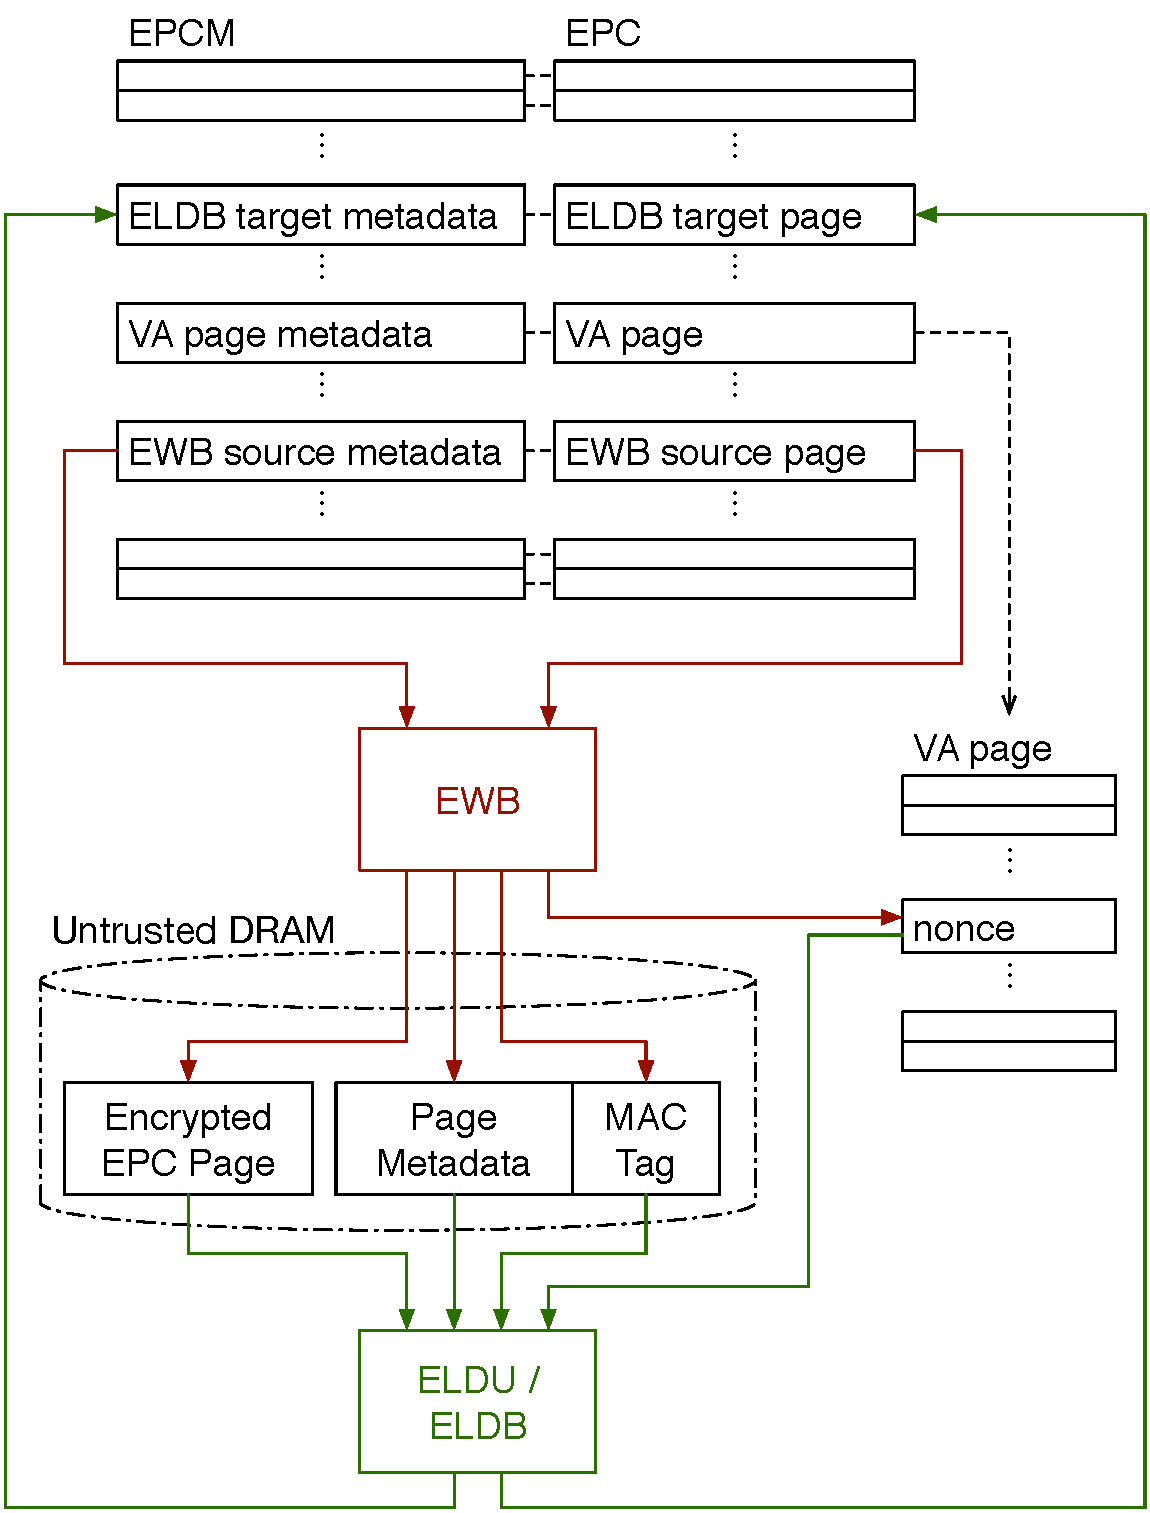
\includegraphics[width=85mm]{figures/sgx_eviction.pdf}
  \caption{
    The \texttt{EWB} instruction outputs the encrypted contents of the
    evicted EPC page, a subset of the fields in the page's EPCM entry, a
    MAC tag, and a nonce. All this information is used by the \texttt{ELDB} or
    \texttt{ELDU} instruction to load the evicted page back into the EPC, with
    privacy, integrity and freshness guarantees.
  }
  \label{fig:sgx_eviction}
\end{figure}

% EWB: SDM S 41.3

\texttt{EWB}'s output consists of an encrypted version of the evicted EPC
page's contents, a subset of the fields in the EPCM entry corresponding to the
page, the nonce discussed in \S~\ref{sec:sgx_va}, and a message authentication
code~(MAC,~\S~\ref{sec:integrity_crypto}) tag. With the exception of the nonce,
\texttt{EWB} writes its output in DRAM outside the PRM area, so the system
software can choose to further evict it to disk.

The EPC page contents is encrypted, to protect the privacy of the enclave's
data while the page is stored in the untrusted DRAM outside the PRM range.
Without the use of encryption, the system software could learn the contents of
an EPC page by evicting it from the EPC.

% Security Information (SECINFO): SDM S 38.11, S 38.11.{1,2}

The page metadata is stored in a \textit{Page Information}~(PAGEINFO)
structure, illustrated in Figure~\ref{fig:sgx_ewb_pageinfo}. This structure is
similar to the PAGEINFO structure described in \S~\ref{sec:sgx_eadd} and
depicted in Figure~\ref{fig:sgx_pageinfo}, except that the SECINFO field has
been replaced by a PCMD field, which contains the virtual address of a
\textit{Page Crypto Metadata}~(PCMD) structure.

\begin{figure}[hbt]
  \centering
  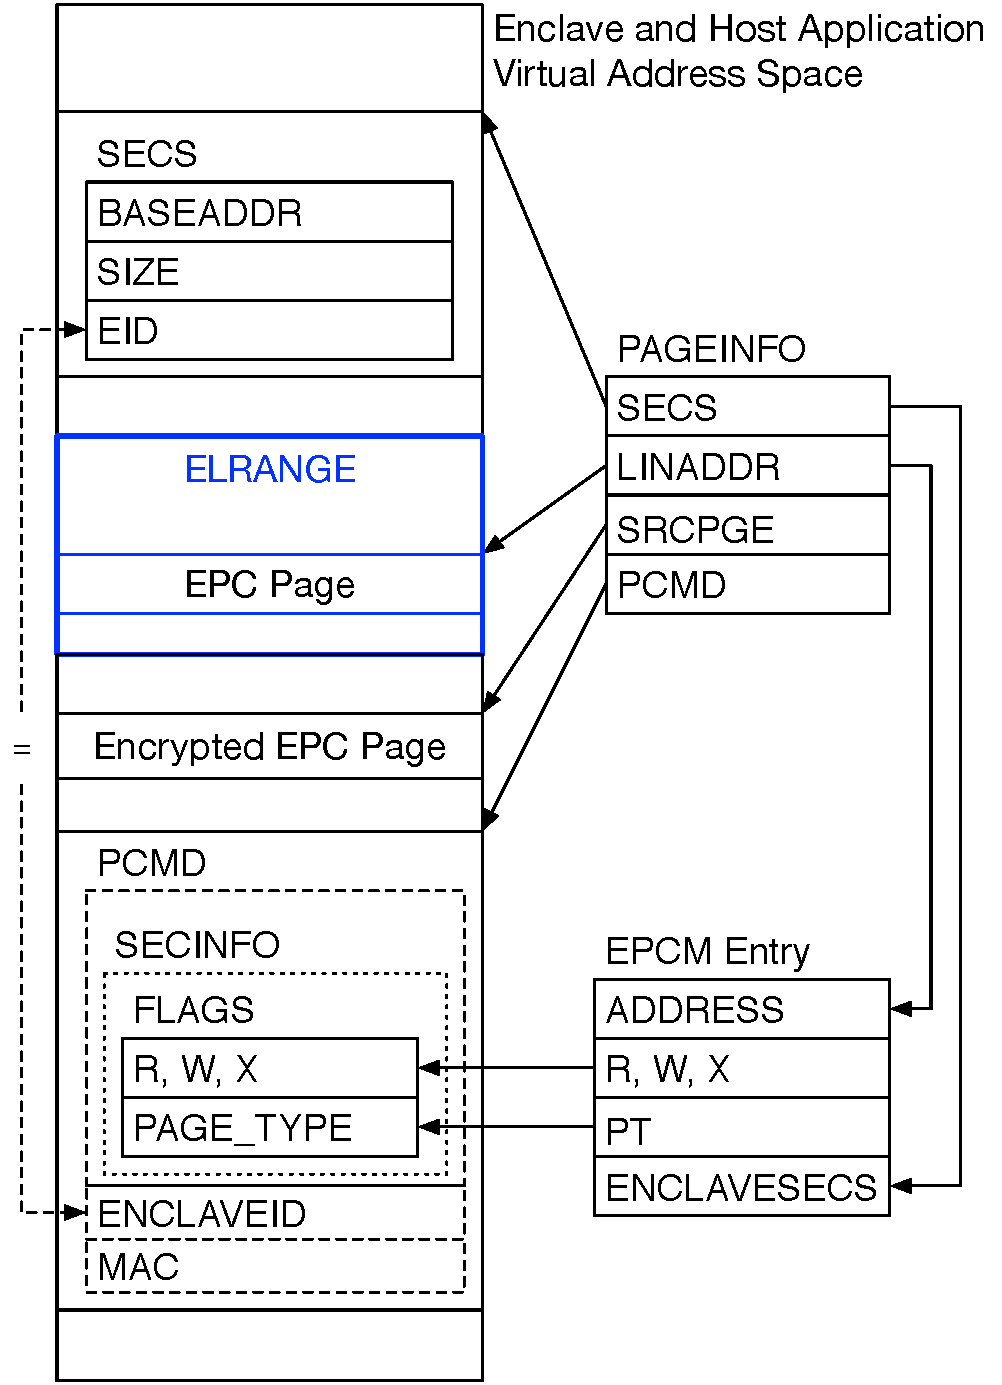
\includegraphics[width=75mm]{figures/sgx_ewb_pageinfo.pdf}
  \caption{
    The PAGEINFO structure used by the \texttt{EWB} and \texttt{ELDU} /
    \texttt{ELDB} instructions
  }
  \label{fig:sgx_ewb_pageinfo}
\end{figure}

The LINADDR field in the PAGEINFO structure is used to store the ADDRESS field
in the EPCM entry, which indicates expected virtual address used to access the
page. The PCMD structure embeds the \textit{Security Information}~(SECINFO)
described in \S~\ref{sec:sgx_eadd}, which is used to store the page type~(PT)
and the access permission flags~(R, W, X) in the EPCM entry. The PCMD structure
also stores the enclave's ID~(EID,~\S~\ref{sec:sgx_eid}). These fields are
later used by \texttt{ELDU} or \texttt{ELDB} to populate the EPCM entry for the
EPC page that is loaded back in.

The metadata described above is stored unencrypted, so the OS has the option of
using the information inside as-is for its own bookkeeping. This has no
negative impact on security, because the metadata is not confidential. In fact,
with the exception of the enclave ID, all the metadata fields are specified by
the system software when \texttt{ECREATE} is called. The enclave ID is only
useful for identifying the enclave that the EPC page belongs to, and the system
software already has this information as well.

Asides from the metadata described above, the PCMD structure also stores the
MAC tag generated by \texttt{EWB}. The MAC tag covers the authenticity of the
EPC page contents, the metadata, and the nonce. The MAC tag is checked by
\texttt{ELDU} and \texttt{ELDB}, which will only load an evicted page back into
the EPC if the MAC verification confirms the authenticity of the page data,
metadata, and nonce. This security check protects against the page swapping
attacks described in \S~\ref{sec:page_swapping_attacks}.

% Eviction of an SECS Page: SDM S 39.5.5

Similarly to \texttt{EREMOVE}, \texttt{EWB} will only evict the EPC page
holding an enclave's SECS if there is no other EPCM entry whose ENCLAVESECS
field references the SECS. At the same time, as an optimization, the SGX
implementation does not perform \texttt{ETRACK}-related checks when evicting a
SECS. This is safe because a SECS is only evicted if the EPC has no pages
belonging to the SECS' enclave, which implies that there isn't any TCS
belonging to the enclave in the EPC, so no processor can be executing enclave
code.

% Eviction of a Version Array Page: SDM S 39.5.6

The pages holding Version Arrays can be evicted, just like any other EPC page.
VA pages are never accessible by software, so they can't have any TLB entries
pointing to them. Therefore, \texttt{EWB} evicts VA pages without performing
any \texttt{ETRACK}-related checks. The ability to evict VA pages has profound
implications that will be discussed in \S~\ref{sec:sgx_eviction_trees}.

\texttt{EWB}'s dataflow, shown in detail in Figure~\ref{fig:sgx_ewb}, has an
aspect that can be confusing to OS developers. The instruction reads the
virtual address of the EPC page to be evicted from a register (RBX) and writes
it to the LINADDR field of the PAGEINFO structure that it is provded. The
separate input (RBX) could have been removed by having the EPC page's address
be provided in the LINADDR field.

\begin{figure}[hbt!]
  \centering
  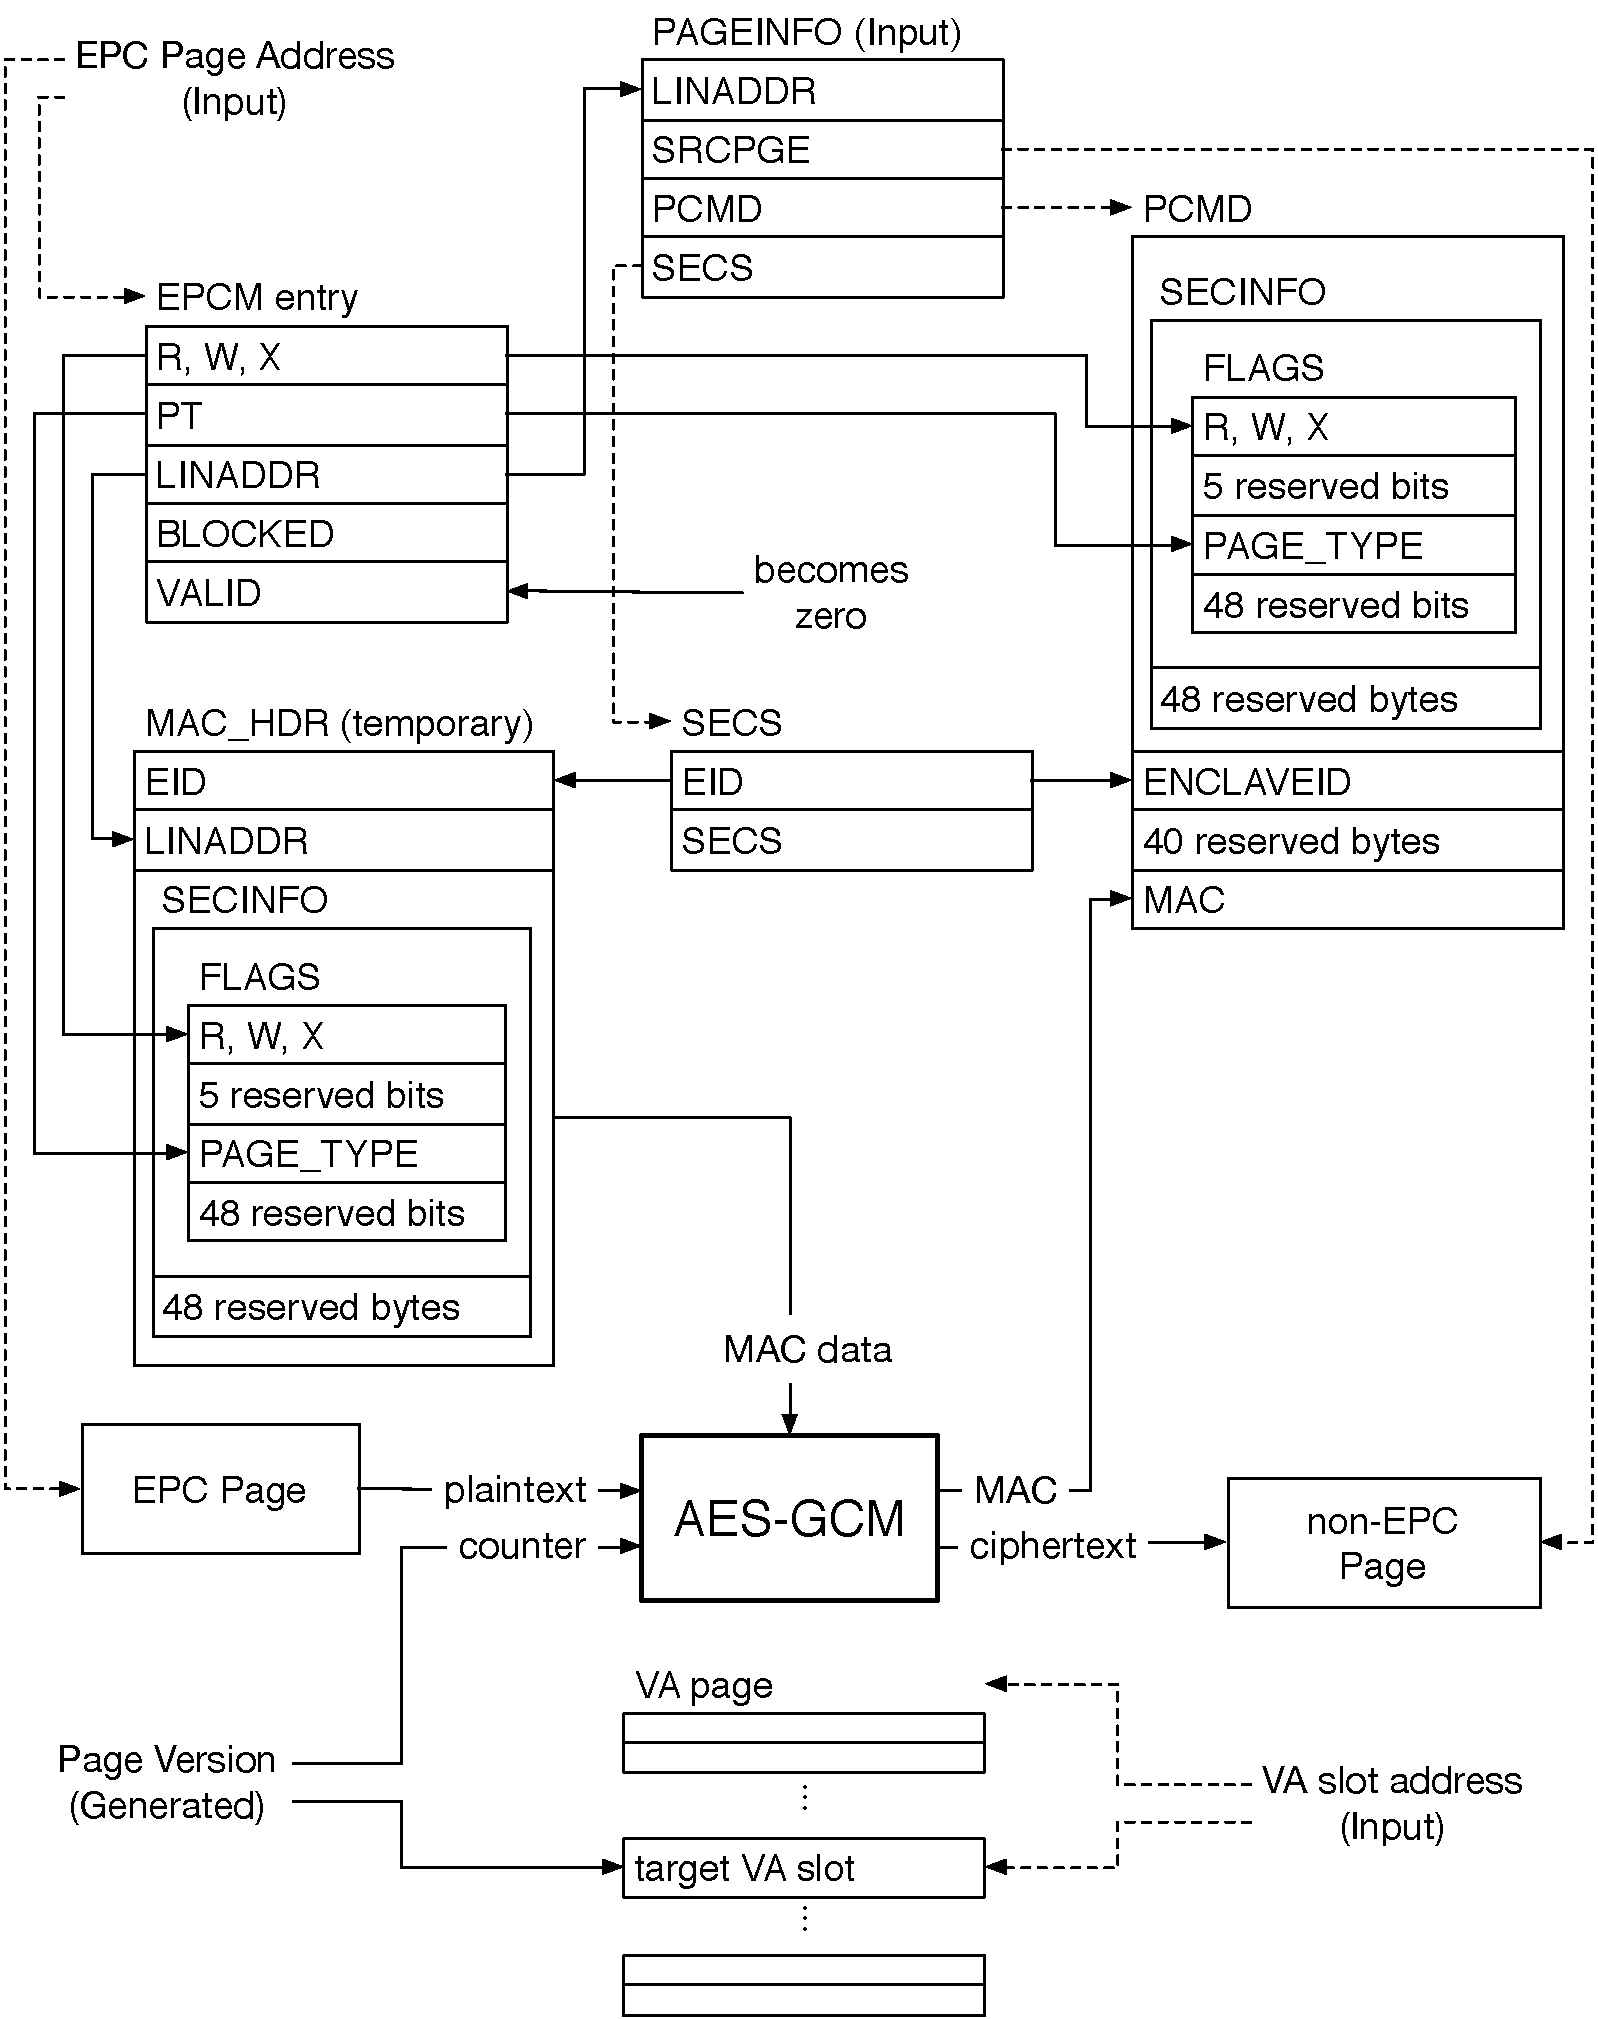
\includegraphics[width=85mm]{figures/sgx_ewb.pdf}
  \caption{
    The data flow of the EWB instruction that evicts an EPC page. The page's
    content is encrypted in a non-EPC RAM page. A nonce is created and saved
    in an empty slot inside a VA page. The page's EPCM metadata and a MAC
    are saved in a separate area in non-EPC memory.
  }
  \label{fig:sgx_ewb}
\end{figure}


\subsubsection{Loading an Evicted Page Back into EPC}

% AEX Operational Detail: SDM S 40.4.1

After an EPC page belonging to an enclave is evicted, any attempt to access the
page from enclave code will result in a Page Fault~(\#PF,~\S~\ref{sec:faults}).
The \#PF will cause the logical processor to exit enclave mode via
AEX~(\S~\ref{sec:aex}), and then invoke the OS kernel's page fault handler.

Page faults receive special handling from the AEX process. While leaving the
enclave, the AEX logic specifically checks if the hardware exception that
triggerred the AEX was \#PF. If that is the case, the AEX implementation clears
the least significant 12 bits of the CR2 register, which stores the virtual
address whose translation caused a page fault.

In general, the OS kernel's page handler needs to be able to extract the
virtual page number~(VPN,~\S~\ref{sec:paging_vpn}) from CR2, so that it knows
which memory page needs to be loaded back into DRAM. The OS kernel may also be
able to use the 12 least signficant address bits, which are not part of the
VPN, to better predict the application software's memory access patterns.
However, unlike the bits that make up the VPN, the bottom 12 bits are not
absolutely necessary for the fault handler to carry out its job. Therefore,
SGX's AEX implementation clears these 12 bits, in order to limit the amount of
information that is learned by the page fault handler.

% Loading an Enclave Page: SDM S 39.5.4
% TODO: page fault -> AEX -> ELDB / ELDU

When the OS page fault handler examines the address in the CR2 register and
determines that the faulting address is inside the EPC, it is generally
expected to use the \texttt{ELDU} or \texttt{ELDB} instruction to load the
evicted page back into the EPC. If the outputs of \texttt{EWB} have been
evicted from DRAM to a slower storage medium, the OS kernel will have to read
the outputs back into DRAM before invoking \texttt{ELDU} / \texttt{ELDB}.

\texttt{ELDU} and \texttt{ELDB} verify the MAC tag produced by \texttt{EWB},
described in \S~\ref{sec:sgx_ewb}. This prevents the OS kernel from performing
the page swapping-based active address translation attack described in
\S~\ref{sec:page_swapping_attacks}.


\subsubsection{Eviction Trees}
\label{sec:sgx_eviction_trees}

The SGX design allows VA pages to be evicted from the EPC, just like enclave
pages. When a VA page is evicted from EPC, all the nonces stored by the VA
slots become inaccessible to the processor. Therefore, the evicted pages
associated with these nonces cannot be restored by \texttt{ELDB} until the
OS loads the VA page back into the EPC.

In other words, an evicted page depends on the VA page storing its nonce, and
cannot be loaded back into the EPC until the VA page is loaded back in as well.
The dependency graph created by this relationship is a forest of
\texttt{eviction trees}. An eviction tree, shown in
Figure~\ref{fig:sgx_eviction_tree}, has enclave EPC pages as leaves, and VA
pages as inner nodes. A page's parent is the VA page that holds its nonce.
Since \texttt{EWB} always outputs a nonce in a VA page, the root node of each
eviction tree is always a VA page in the EPC.

\begin{figure}[hbt!]
  \centering
  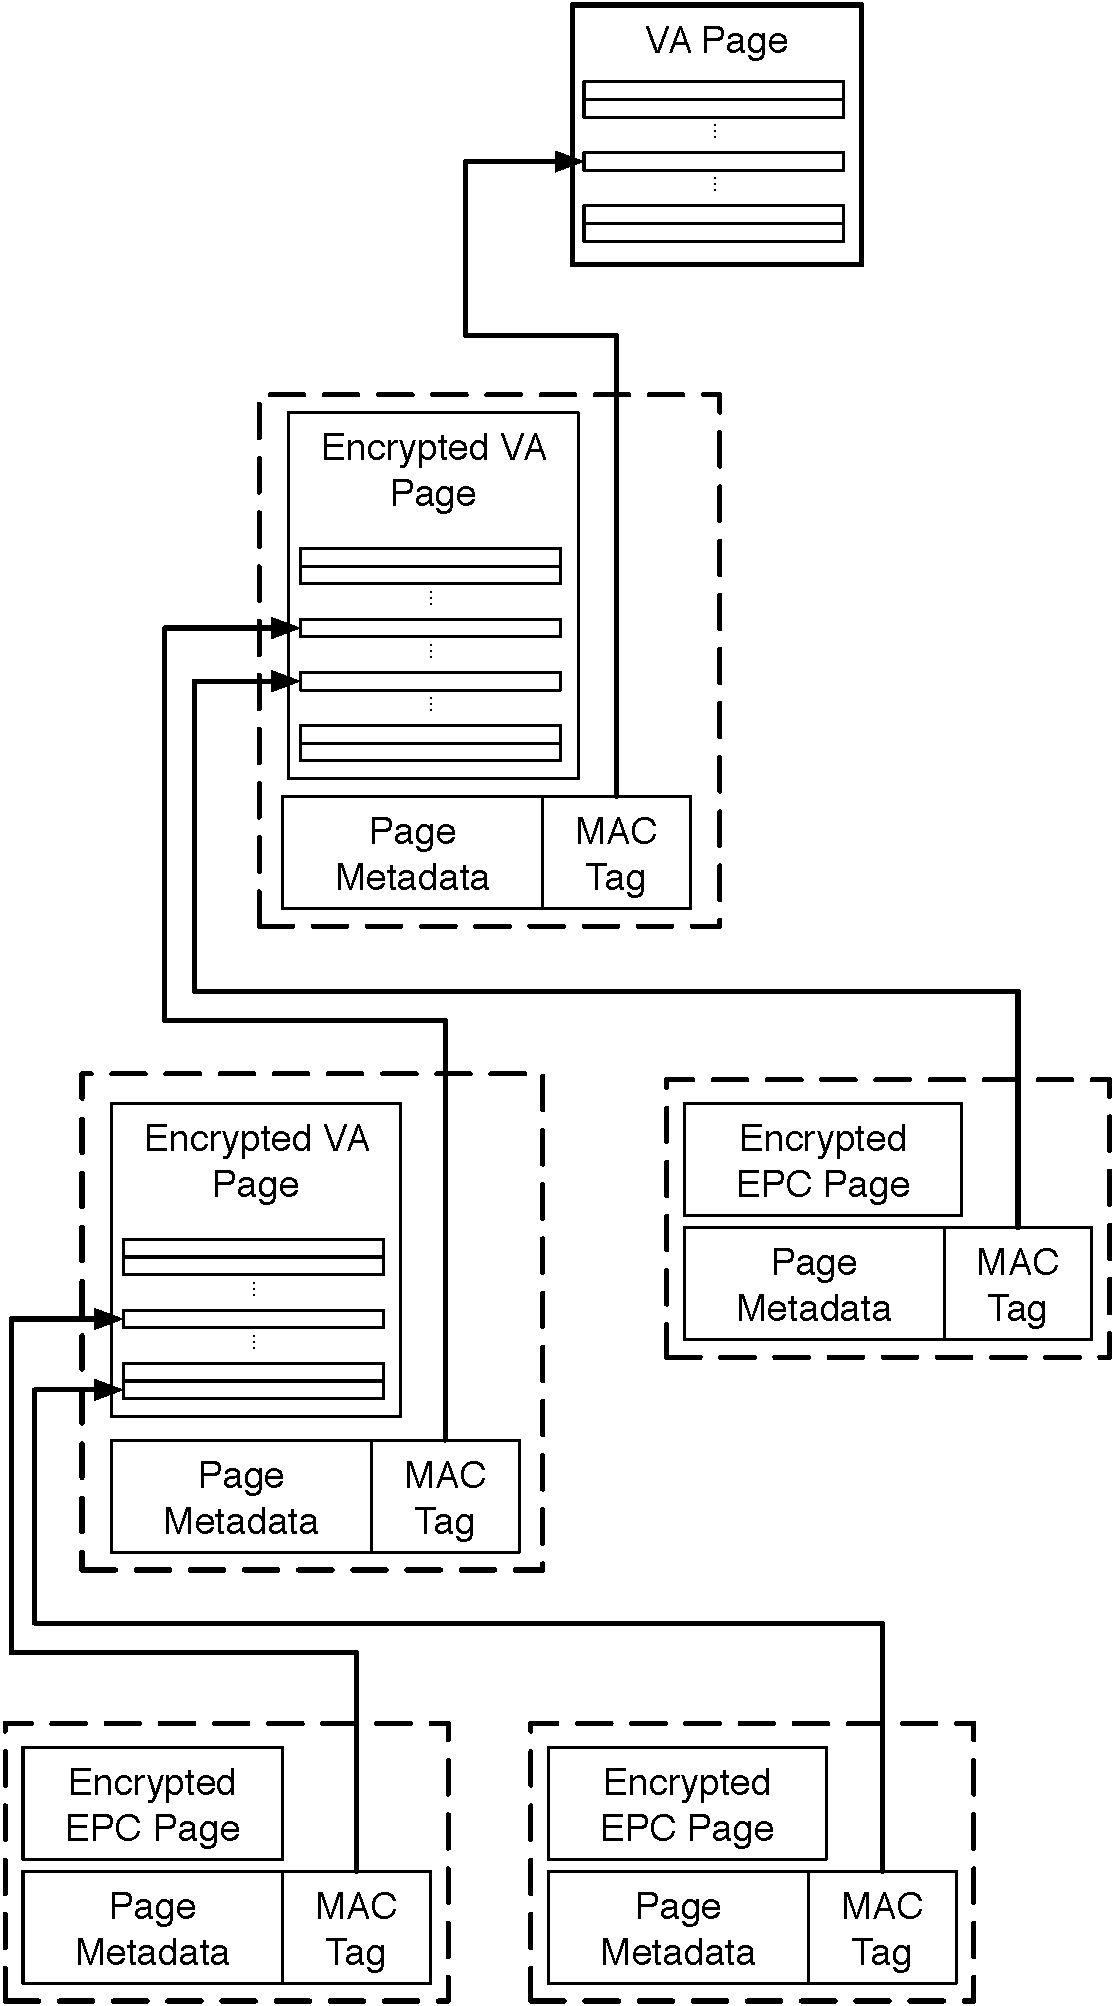
\includegraphics[width=80mm]{figures/sgx_eviction_tree.pdf}
  \caption{
    A version tree formed by evicted VA pages and enclave EPC pages. The
    enclave pages are leaves, and the VA pages are inner nodes. The OS controls
    the tree's shape, which impacts the performance of evictions, but not their
    correctness.
  }
  \label{fig:sgx_eviction_tree}
\end{figure}

A straightforward inductive argument shows that when an OS wishes to load an
evicted enclave page back into the EPC, it needs to load all the VA pages on
the path from the eviction tree's root to the leaf corresponding to the enclave
page. Therefore, the number of page loads required to satisfy a page fault
inside the EPC depends on the shape of the eviction tree that contains the
page.

The SGX design leaves the OS in complete control of the shape of the eviction
trees. This has no negative impact on security, as the tree shape only impacts
the performance of the eviction scheme, and not its correctness.
